% !TEX program = xelatex
\documentclass[twocolumn,superscriptaddress,english,showpacs,longbibliography]{revtex4-2}
\usepackage[colorlinks=true,urlcolor=blue,citecolor=blue,linkcolor=blue]{hyperref} 

\usepackage{svg}
\usepackage{amsmath}
\usepackage{graphicx}% Include figure files
\usepackage{textcomp}
\usepackage{bm}% bold math
\usepackage{color}
\usepackage{amssymb}
\usepackage{graphicx}
\usepackage{color}
\usepackage{mathrsfs}
\usepackage{float}
\usepackage{indentfirst}
\usepackage{txfonts}
\usepackage{algorithm}  
\usepackage{algpseudocode}  
\usepackage{balance}
\usepackage{flushend}
\usepackage{cleveref}
\usepackage{tikz}
\renewcommand{\algorithmicrequire}{\textbf{Input:}}  % Use Input in the format of Algorithm  
\renewcommand{\algorithmicensure}{\textbf{Output:}} % Use Output in the format of Algorithm  


\newcommand{\jgl}[1]{[{\color{green}{JGL: #1}}]}
\newcommand{\s}{\mathbf {s}}
\newcommand{\net}[1]{{\textsc{#1}}}
\newcommand{\argmin}{\mathop{\mathrm{argmin}}\limits}
\newcommand{\Eq}[1]{Eq.~(\ref{#1})}
\newcommand{\Fig}[1]{Fig.~\ref{#1}}

\begin{document}

\title{Surface programmable materials}

\author{Authors}
\email{xxx@xxx.com}
\affiliation{
    XXX
}

\begin{abstract}
\end{abstract}

\maketitle

\section{Introduction}

\textbf{Definition: (Surface programmable material)}: a lattice (with
translational invariance) model that can be programmed on its surfaces
to perform universal computation.

\section{Model and Method}
\subsection{Elementary cellular automaton}\label{elementary-cellular-automaton}

An elementary cellular automaton is a 1-dimensional cellular
automaton, where there are two possible states (labeled by 0 and 1). The rule to
determine the state of the cell in next generation depends only on the
current state of the cell and its two immediate neighbors.

There are $8 = 2^3$ possible configurations for a cell and its two
immediate neighbors. Different elementary cellular automaton are only
different from their translation rules. There are only $2^8 = 256$
different rules, so do the automatons.

If we put each possible current configurations in order: 111, 110,
\ldots, 001, 000, and put the resulting state under them. We then get an
integer in its binary representations. Then this integer is taken to be
the rule number of the automaton. For example, rule 110.

Given that $110_d = 01101110_2$, so rule 110 is defined by the
translation rule:

\begin{tabular}{|c|c|c|c|c|c|c|c|c|}
\hline
Current Pattern & 111 & 110 & 101 & 100 & 011 & 010 & 001 & 000 \\
\hline
New Center Cell & 0 & 1 & 1 & 0 & 1 & 1 & 1 & 0 \\
\hline
\end{tabular}

Rule 110 has been shown to be Turing Complete~\cite{Cook2009}, and thus capable of universal
computation.

\subsection{Energy model}\label{a-2d-surface-programmable-material}

Let us define a model Hamiltonian on a 2D lattice as
\begin{equation}\label{eq:toy-hamiltonian}
H = \sum_{\text{each gadget}} (n_{i+1, t} \land \neg(n_{i, t} \land \neg n_{i-1, t})) \veebar n_{i,t+1},
\end{equation}
where $n_{i, t} \in \{0, 1\}$ is the state of the cell at row $i$ and column $t$.
Its ground state with energy $0$ encodes a $110$ cellular automaton, where the direction of computation is from the left to right.

The gadget we constructed based on the Rule 110 cellular automaton
naturally possesses Turing completeness. Therefore, it can be tiled in a
two-dimensional plane to create a computational material with logical
operation capabilities.

\tikzset{every picture/.style={line width=0.75pt}} %set default line width to 0.75pt        

\begin{center}
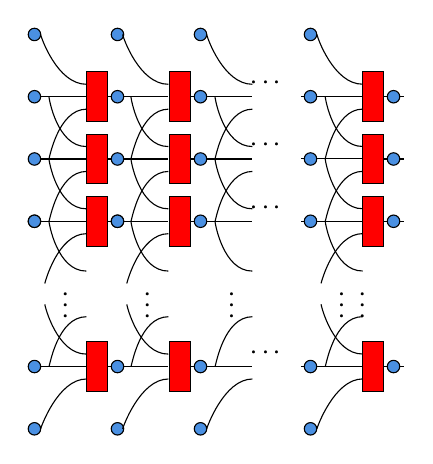
\begin{tikzpicture}[x=0.75pt,y=0.75pt,yscale=-1,xscale=1]
%uncomment if require: \path (0,300); %set diagram left start at 0, and has height of 300

%Shape: Square [id:dp3257799447745866] 
\draw  [fill={rgb, 255:red, 255; green, 0; blue, 0 }  ,fill opacity=1 ] (30,30) -- (40,30) -- (40,54) -- (30,54) -- cycle ;
%Straight Lines [id:da8913459345633652] 
\draw    (20,42) -- (30,42) ;
%Straight Lines [id:da9790784501640646] 
\draw    (40,42) -- (60,42) ;
%Shape: Square [id:dp5326406990508012] 
\draw  [fill={rgb, 255:red, 255; green, 0; blue, 0 }  ,fill opacity=1 ] (70,30) -- (80,30) -- (80,54) -- (70,54) -- cycle ;
%Straight Lines [id:da008320062158621688] 
\draw    (80,42) -- (100,42) ;
%Shape: Square [id:dp29003962631292124] 
\draw  [fill={rgb, 255:red, 255; green, 0; blue, 0 }  ,fill opacity=1 ] (30,60) -- (40,60) -- (40,84) -- (30,84) -- cycle ;
%Straight Lines [id:da8695035786947396] 
\draw    (20,72) -- (30,72) ;
%Straight Lines [id:da417768427429108] 
\draw    (40,72) -- (60,72) ;
%Shape: Square [id:dp08018354727485644] 
\draw  [fill={rgb, 255:red, 255; green, 0; blue, 0 }  ,fill opacity=1 ] (70,60) -- (80,60) -- (80,84) -- (70,84) -- cycle ;
%Straight Lines [id:da7038299022670145] 
\draw    (80,72) -- (100,72) ;
%Shape: Square [id:dp4665291997770109] 
\draw  [fill={rgb, 255:red, 255; green, 0; blue, 0 }  ,fill opacity=1 ] (30,90) -- (40,90) -- (40,114) -- (30,114) -- cycle ;
%Straight Lines [id:da9280920191618629] 
\draw    (20,102) -- (30,102) ;
%Straight Lines [id:da023978392575592755] 
\draw    (40,102) -- (60,102) ;
%Shape: Square [id:dp9172017959293151] 
\draw  [fill={rgb, 255:red, 255; green, 0; blue, 0 }  ,fill opacity=1 ] (70,90) -- (80,90) -- (80,114) -- (70,114) -- cycle ;
%Straight Lines [id:da515300595667447] 
\draw    (80,102) -- (100,102) ;
%Straight Lines [id:da9288304396586808] 
\draw    (80,72) -- (100,72) ;
%Straight Lines [id:da852280866297966] 
\draw    (80,102) -- (100,102) ;
%Shape: Square [id:dp32738689596333903] 
\draw  [fill={rgb, 255:red, 255; green, 0; blue, 0 }  ,fill opacity=1 ] (30,160) -- (40,160) -- (40,184) -- (30,184) -- cycle ;
%Straight Lines [id:da07485978922844372] 
\draw    (20,172) -- (30,172) ;
%Straight Lines [id:da2475700164417307] 
\draw    (40,172) -- (60,172) ;
%Shape: Square [id:dp4553302503149699] 
\draw  [fill={rgb, 255:red, 255; green, 0; blue, 0 }  ,fill opacity=1 ] (70,160) -- (80,160) -- (80,184) -- (70,184) -- cycle ;
%Straight Lines [id:da5669313532997795] 
\draw    (80,172) -- (100,172) ;
%Shape: Square [id:dp681519742049937] 
\draw  [fill={rgb, 255:red, 255; green, 0; blue, 0 }  ,fill opacity=1 ] (163,30) -- (173,30) -- (173,54) -- (163,54) -- cycle ;
%Shape: Square [id:dp2901897648605303] 
\draw  [fill={rgb, 255:red, 255; green, 0; blue, 0 }  ,fill opacity=1 ] (163,60) -- (173,60) -- (173,84) -- (163,84) -- cycle ;
%Shape: Square [id:dp9710219091133365] 
\draw  [fill={rgb, 255:red, 255; green, 0; blue, 0 }  ,fill opacity=1 ] (163,90) -- (173,90) -- (173,114) -- (163,114) -- cycle ;
%Shape: Square [id:dp47295881968788644] 
\draw  [fill={rgb, 255:red, 255; green, 0; blue, 0 }  ,fill opacity=1 ] (163,160) -- (173,160) -- (173,184) -- (163,184) -- cycle ;
%Straight Lines [id:da1585638759400958] 
\draw    (173,172) -- (183,172) ;
%Straight Lines [id:da5795532995572801] 
\draw    (173,102) -- (183,102) ;
%Straight Lines [id:da8448651727682703] 
\draw    (173,72) -- (183,72) ;
%Straight Lines [id:da9060816552835422] 
\draw    (173,42) -- (183,42) ;
%Shape: Circle [id:dp818609500871543] 
\draw  [fill={rgb, 255:red, 74; green, 144; blue, 226 }  ,fill opacity=1 ] (42,42) .. controls (42,40.34) and (43.34,39) .. (45,39) .. controls (46.66,39) and (48,40.34) .. (48,42) .. controls (48,43.66) and (46.66,45) .. (45,45) .. controls (43.34,45) and (42,43.66) .. (42,42) -- cycle ;
%Shape: Circle [id:dp13831345755639668] 
\draw  [fill={rgb, 255:red, 74; green, 144; blue, 226 }  ,fill opacity=1 ] (42,72) .. controls (42,70.34) and (43.34,69) .. (45,69) .. controls (46.66,69) and (48,70.34) .. (48,72) .. controls (48,73.66) and (46.66,75) .. (45,75) .. controls (43.34,75) and (42,73.66) .. (42,72) -- cycle ;
%Shape: Circle [id:dp9041445092942773] 
\draw   (42,102) .. controls (42,100.34) and (43.34,99) .. (45,99) .. controls (46.66,99) and (48,100.34) .. (48,102) .. controls (48,103.66) and (46.66,105) .. (45,105) .. controls (43.34,105) and (42,103.66) .. (42,102) -- cycle ;
%Shape: Circle [id:dp7529245942690144] 
\draw  [fill={rgb, 255:red, 74; green, 144; blue, 226 }  ,fill opacity=1 ] (42,172) .. controls (42,170.34) and (43.34,169) .. (45,169) .. controls (46.66,169) and (48,170.34) .. (48,172) .. controls (48,173.66) and (46.66,175) .. (45,175) .. controls (43.34,175) and (42,173.66) .. (42,172) -- cycle ;
%Shape: Circle [id:dp4421700288524639] 
\draw  [fill={rgb, 255:red, 74; green, 144; blue, 226 }  ,fill opacity=1 ] (82,172) .. controls (82,170.34) and (83.34,169) .. (85,169) .. controls (86.66,169) and (88,170.34) .. (88,172) .. controls (88,173.66) and (86.66,175) .. (85,175) .. controls (83.34,175) and (82,173.66) .. (82,172) -- cycle ;
%Shape: Circle [id:dp4431783957619826] 
\draw  [fill={rgb, 255:red, 74; green, 144; blue, 226 }  ,fill opacity=1 ] (82,102) .. controls (82,100.34) and (83.34,99) .. (85,99) .. controls (86.66,99) and (88,100.34) .. (88,102) .. controls (88,103.66) and (86.66,105) .. (85,105) .. controls (83.34,105) and (82,103.66) .. (82,102) -- cycle ;
%Shape: Circle [id:dp403539897070186] 
\draw  [fill={rgb, 255:red, 74; green, 144; blue, 226 }  ,fill opacity=1 ] (42,102) .. controls (42,100.34) and (43.34,99) .. (45,99) .. controls (46.66,99) and (48,100.34) .. (48,102) .. controls (48,103.66) and (46.66,105) .. (45,105) .. controls (43.34,105) and (42,103.66) .. (42,102) -- cycle ;
%Shape: Circle [id:dp8783887479009327] 
\draw  [fill={rgb, 255:red, 74; green, 144; blue, 226 }  ,fill opacity=1 ] (82,72) .. controls (82,70.34) and (83.34,69) .. (85,69) .. controls (86.66,69) and (88,70.34) .. (88,72) .. controls (88,73.66) and (86.66,75) .. (85,75) .. controls (83.34,75) and (82,73.66) .. (82,72) -- cycle ;
%Shape: Circle [id:dp6224124506773947] 
\draw  [fill={rgb, 255:red, 74; green, 144; blue, 226 }  ,fill opacity=1 ] (82,42) .. controls (82,40.34) and (83.34,39) .. (85,39) .. controls (86.66,39) and (88,40.34) .. (88,42) .. controls (88,43.66) and (86.66,45) .. (85,45) .. controls (83.34,45) and (82,43.66) .. (82,42) -- cycle ;
%Shape: Circle [id:dp8043981259851258] 
\draw  [fill={rgb, 255:red, 74; green, 144; blue, 226 }  ,fill opacity=1 ] (175,102) .. controls (175,100.34) and (176.34,99) .. (178,99) .. controls (179.66,99) and (181,100.34) .. (181,102) .. controls (181,103.66) and (179.66,105) .. (178,105) .. controls (176.34,105) and (175,103.66) .. (175,102) -- cycle ;
%Shape: Circle [id:dp43816466417546707] 
\draw  [fill={rgb, 255:red, 74; green, 144; blue, 226 }  ,fill opacity=1 ] (175,172) .. controls (175,170.34) and (176.34,169) .. (178,169) .. controls (179.66,169) and (181,170.34) .. (181,172) .. controls (181,173.66) and (179.66,175) .. (178,175) .. controls (176.34,175) and (175,173.66) .. (175,172) -- cycle ;
%Shape: Circle [id:dp5620143122025991] 
\draw  [fill={rgb, 255:red, 74; green, 144; blue, 226 }  ,fill opacity=1 ] (175,72) .. controls (175,70.34) and (176.34,69) .. (178,69) .. controls (179.66,69) and (181,70.34) .. (181,72) .. controls (181,73.66) and (179.66,75) .. (178,75) .. controls (176.34,75) and (175,73.66) .. (175,72) -- cycle ;
%Shape: Circle [id:dp8865997979090963] 
\draw  [fill={rgb, 255:red, 74; green, 144; blue, 226 }  ,fill opacity=1 ] (175,42) .. controls (175,40.34) and (176.34,39) .. (178,39) .. controls (179.66,39) and (181,40.34) .. (181,42) .. controls (181,43.66) and (179.66,45) .. (178,45) .. controls (176.34,45) and (175,43.66) .. (175,42) -- cycle ;
%Shape: Circle [id:dp18306264726647137] 
\draw  [fill={rgb, 255:red, 74; green, 144; blue, 226 }  ,fill opacity=1 ] (42,202) .. controls (42,200.34) and (43.34,199) .. (45,199) .. controls (46.66,199) and (48,200.34) .. (48,202) .. controls (48,203.66) and (46.66,205) .. (45,205) .. controls (43.34,205) and (42,203.66) .. (42,202) -- cycle ;
%Shape: Circle [id:dp3243993178712161] 
\draw  [fill={rgb, 255:red, 74; green, 144; blue, 226 }  ,fill opacity=1 ] (42,12) .. controls (42,10.34) and (43.34,9) .. (45,9) .. controls (46.66,9) and (48,10.34) .. (48,12) .. controls (48,13.66) and (46.66,15) .. (45,15) .. controls (43.34,15) and (42,13.66) .. (42,12) -- cycle ;
%Shape: Circle [id:dp3529141461836287] 
\draw  [fill={rgb, 255:red, 74; green, 144; blue, 226 }  ,fill opacity=1 ] (135,12) .. controls (135,10.34) and (136.34,9) .. (138,9) .. controls (139.66,9) and (141,10.34) .. (141,12) .. controls (141,13.66) and (139.66,15) .. (138,15) .. controls (136.34,15) and (135,13.66) .. (135,12) -- cycle ;
%Shape: Circle [id:dp9431375452836528] 
\draw  [fill={rgb, 255:red, 74; green, 144; blue, 226 }  ,fill opacity=1 ] (135,202) .. controls (135,200.34) and (136.34,199) .. (138,199) .. controls (139.66,199) and (141,200.34) .. (141,202) .. controls (141,203.66) and (139.66,205) .. (138,205) .. controls (136.34,205) and (135,203.66) .. (135,202) -- cycle ;
%Straight Lines [id:da9696356596865732] 
\draw    (5,42) -- (20,42) ;
%Straight Lines [id:da5317592058087168] 
\draw    (5,72) -- (20,72) ;
%Straight Lines [id:da6169293205402535] 
\draw    (5,102) -- (20,102) ;
%Straight Lines [id:da9653690034485647] 
\draw    (5,172) -- (20,172) ;
%Shape: Circle [id:dp11541023046031418] 
\draw  [fill={rgb, 255:red, 74; green, 144; blue, 226 }  ,fill opacity=1 ] (2,42) .. controls (2,40.34) and (3.34,39) .. (5,39) .. controls (6.66,39) and (8,40.34) .. (8,42) .. controls (8,43.66) and (6.66,45) .. (5,45) .. controls (3.34,45) and (2,43.66) .. (2,42) -- cycle ;
%Shape: Circle [id:dp9967907554667488] 
\draw  [fill={rgb, 255:red, 74; green, 144; blue, 226 }  ,fill opacity=1 ] (2,72) .. controls (2,70.34) and (3.34,69) .. (5,69) .. controls (6.66,69) and (8,70.34) .. (8,72) .. controls (8,73.66) and (6.66,75) .. (5,75) .. controls (3.34,75) and (2,73.66) .. (2,72) -- cycle ;
%Shape: Circle [id:dp5466737045582317] 
\draw   (2,102) .. controls (2,100.34) and (3.34,99) .. (5,99) .. controls (6.66,99) and (8,100.34) .. (8,102) .. controls (8,103.66) and (6.66,105) .. (5,105) .. controls (3.34,105) and (2,103.66) .. (2,102) -- cycle ;
%Shape: Circle [id:dp22351697734701603] 
\draw  [fill={rgb, 255:red, 74; green, 144; blue, 226 }  ,fill opacity=1 ] (2,172) .. controls (2,170.34) and (3.34,169) .. (5,169) .. controls (6.66,169) and (8,170.34) .. (8,172) .. controls (8,173.66) and (6.66,175) .. (5,175) .. controls (3.34,175) and (2,173.66) .. (2,172) -- cycle ;
%Shape: Circle [id:dp07423205757027329] 
\draw  [fill={rgb, 255:red, 74; green, 144; blue, 226 }  ,fill opacity=1 ] (2,102) .. controls (2,100.34) and (3.34,99) .. (5,99) .. controls (6.66,99) and (8,100.34) .. (8,102) .. controls (8,103.66) and (6.66,105) .. (5,105) .. controls (3.34,105) and (2,103.66) .. (2,102) -- cycle ;
%Shape: Circle [id:dp44591669371444054] 
\draw  [fill={rgb, 255:red, 74; green, 144; blue, 226 }  ,fill opacity=1 ] (2,202) .. controls (2,200.34) and (3.34,199) .. (5,199) .. controls (6.66,199) and (8,200.34) .. (8,202) .. controls (8,203.66) and (6.66,205) .. (5,205) .. controls (3.34,205) and (2,203.66) .. (2,202) -- cycle ;
%Shape: Circle [id:dp8124810079347506] 
\draw  [fill={rgb, 255:red, 74; green, 144; blue, 226 }  ,fill opacity=1 ] (2,12) .. controls (2,10.34) and (3.34,9) .. (5,9) .. controls (6.66,9) and (8,10.34) .. (8,12) .. controls (8,13.66) and (6.66,15) .. (5,15) .. controls (3.34,15) and (2,13.66) .. (2,12) -- cycle ;
%Curve Lines [id:da6837659640523519] 
\draw    (12,72) .. controls (11.9,72.82) and (16.25,48.02) .. (30,48) ;
%Curve Lines [id:da14157714470554095] 
\draw    (12,102) .. controls (12.25,102.02) and (16.25,78.02) .. (30,78) ;
%Curve Lines [id:da29397752720095016] 
\draw    (10,132) .. controls (9.9,131.92) and (16.25,108.02) .. (30,108) ;
%Curve Lines [id:da1010168964172955] 
\draw    (8,202) .. controls (7.88,201.94) and (16.25,178.02) .. (30,178) ;
%Curve Lines [id:da41907939317602727] 
\draw    (30,66) .. controls (15.95,66.07) and (11.95,42.82) .. (12,42) ;
%Curve Lines [id:da4960426207730133] 
\draw    (30,96) .. controls (15.95,96.07) and (11.95,72.82) .. (12,72) ;
%Curve Lines [id:da32194834856252696] 
\draw    (30,126) .. controls (15.95,126.07) and (11.95,102.82) .. (12,102) ;
%Curve Lines [id:da9942559529163806] 
\draw    (30,166) .. controls (15.95,166.07) and (9.95,142.82) .. (10,142) ;
%Curve Lines [id:da30812169087400987] 
\draw    (30,36) .. controls (15.95,36.07) and (7.95,12.82) .. (8,12) ;
%Curve Lines [id:da7415436207281032] 
\draw    (12,172) .. controls (12.4,171.42) and (16.25,148.02) .. (30,148) ;
%Straight Lines [id:da945225908298071] 
\draw    (59.5,42) -- (69.5,42) ;
%Straight Lines [id:da019486859954932045] 
\draw    (59.5,72) -- (69.5,72) ;
%Straight Lines [id:da10691701544026788] 
\draw    (59.5,102) -- (69.5,102) ;
%Straight Lines [id:da08190608552147682] 
\draw    (59.5,172) -- (69.5,172) ;
%Straight Lines [id:da5383715063718815] 
\draw    (48,42) -- (59.5,42) ;
%Straight Lines [id:da29185686612996165] 
\draw    (48,72) -- (59.5,72) ;
%Straight Lines [id:da6312076314118666] 
\draw    (48,102) -- (59.5,102) ;
%Straight Lines [id:da0122276432828059] 
\draw    (48,172) -- (59.5,172) ;
%Curve Lines [id:da634843349549117] 
\draw    (51.5,72) .. controls (51.4,72.82) and (55.75,48.02) .. (69.5,48) ;
%Curve Lines [id:da29334484540724026] 
\draw    (51.5,102) .. controls (51.75,102.02) and (55.75,78.02) .. (69.5,78) ;
%Curve Lines [id:da3089090169112314] 
\draw    (49.5,132) .. controls (49.4,131.92) and (55.75,108.02) .. (69.5,108) ;
%Curve Lines [id:da24605443838188257] 
\draw    (47.5,202) .. controls (47.38,201.94) and (55.75,178.02) .. (69.5,178) ;
%Curve Lines [id:da497728473744927] 
\draw    (69.5,66) .. controls (55.45,66.07) and (51.45,42.82) .. (51.5,42) ;
%Curve Lines [id:da1733603989545598] 
\draw    (69.5,96) .. controls (55.45,96.07) and (51.45,72.82) .. (51.5,72) ;
%Curve Lines [id:da7391016400644088] 
\draw    (69.5,126) .. controls (55.45,126.07) and (51.45,102.82) .. (51.5,102) ;
%Curve Lines [id:da2610882313501728] 
\draw    (69.5,166) .. controls (55.45,166.07) and (49.45,142.82) .. (49.5,142) ;
%Curve Lines [id:da9723708662465751] 
\draw    (69.5,36) .. controls (55.45,36.07) and (47.45,12.82) .. (47.5,12) ;
%Curve Lines [id:da7225849641270694] 
\draw    (51.5,172) .. controls (51.9,171.42) and (55.75,148.02) .. (69.5,148) ;
%Straight Lines [id:da7791377752665631] 
\draw    (100,42) -- (110,42) ;
%Straight Lines [id:da23522073116206266] 
\draw    (100,72) -- (110,72) ;
%Straight Lines [id:da18218908732788264] 
\draw    (100,102) -- (110,102) ;
%Straight Lines [id:da3309320538017131] 
\draw    (100,172) -- (110,172) ;
%Straight Lines [id:da4610992726495633] 
\draw    (88,42) -- (100,42) ;
%Straight Lines [id:da1358122827839865] 
\draw    (88,72) -- (100,72) ;
%Straight Lines [id:da9749891373044985] 
\draw    (88,102) -- (100,102) ;
%Straight Lines [id:da6902822758606824] 
\draw    (88,172) -- (100,172) ;
%Curve Lines [id:da8937700604447827] 
\draw    (92,72) .. controls (91.9,72.82) and (96.25,48.02) .. (110,48) ;
%Curve Lines [id:da3731849249187291] 
\draw    (92,102) .. controls (92.25,102.02) and (96.25,78.02) .. (110,78) ;
%Curve Lines [id:da9742316406042617] 
\draw    (88,202) .. controls (87.88,201.94) and (96.25,178.02) .. (110,178) ;
%Curve Lines [id:da6734623491912421] 
\draw    (110,66) .. controls (95.95,66.07) and (91.95,42.82) .. (92,42) ;
%Curve Lines [id:da9728942718366658] 
\draw    (110,96) .. controls (95.95,96.07) and (91.95,72.82) .. (92,72) ;
%Curve Lines [id:da5314963895208473] 
\draw    (110,126) .. controls (95.95,126.07) and (91.95,102.82) .. (92,102) ;
%Curve Lines [id:da20527729986926668] 
\draw    (110,36) .. controls (95.95,36.07) and (87.95,12.82) .. (88,12) ;
%Curve Lines [id:da9357477032373158] 
\draw    (92,172) .. controls (92.4,171.42) and (96.25,148.02) .. (110,148) ;
%Shape: Circle [id:dp03524070526370693] 
\draw  [fill={rgb, 255:red, 74; green, 144; blue, 226 }  ,fill opacity=1 ] (82,12) .. controls (82,10.34) and (83.34,9) .. (85,9) .. controls (86.66,9) and (88,10.34) .. (88,12) .. controls (88,13.66) and (86.66,15) .. (85,15) .. controls (83.34,15) and (82,13.66) .. (82,12) -- cycle ;
%Shape: Circle [id:dp5282167504002355] 
\draw  [fill={rgb, 255:red, 74; green, 144; blue, 226 }  ,fill opacity=1 ] (82,202) .. controls (82,200.34) and (83.34,199) .. (85,199) .. controls (86.66,199) and (88,200.34) .. (88,202) .. controls (88,203.66) and (86.66,205) .. (85,205) .. controls (83.34,205) and (82,203.66) .. (82,202) -- cycle ;
%Straight Lines [id:da28818147273527717] 
\draw    (133.6,41.96) -- (153.6,41.96) ;
%Straight Lines [id:da4792679687432131] 
\draw    (133.6,71.96) -- (153.6,71.96) ;
%Straight Lines [id:da2794298478395634] 
\draw    (133.6,101.96) -- (153.6,101.96) ;
%Straight Lines [id:da610925391950311] 
\draw    (133.6,171.96) -- (153.6,171.96) ;
%Straight Lines [id:da31436080279800227] 
\draw    (153.1,41.96) -- (163.1,41.96) ;
%Straight Lines [id:da07642255702447143] 
\draw    (153.1,71.96) -- (163.1,71.96) ;
%Straight Lines [id:da48431709040149795] 
\draw    (153.1,101.96) -- (163.1,101.96) ;
%Straight Lines [id:da31077160308421736] 
\draw    (153.1,171.96) -- (163.1,171.96) ;
%Straight Lines [id:da4482666583263508] 
\draw    (141.6,41.96) -- (153.1,41.96) ;
%Straight Lines [id:da0031324911441572567] 
\draw    (141.6,71.96) -- (153.1,71.96) ;
%Straight Lines [id:da39186514465416056] 
\draw    (141.6,101.96) -- (153.1,101.96) ;
%Straight Lines [id:da9984443909601395] 
\draw    (141.6,171.96) -- (153.1,171.96) ;
%Curve Lines [id:da2794596982451869] 
\draw    (145.1,71.96) .. controls (145,72.79) and (149.35,47.99) .. (163.1,47.96) ;
%Curve Lines [id:da5527279625811088] 
\draw    (145.1,101.96) .. controls (145.35,101.99) and (149.35,77.99) .. (163.1,77.96) ;
%Curve Lines [id:da49469050221037403] 
\draw    (143.1,131.96) .. controls (143,131.89) and (149.35,107.99) .. (163.1,107.96) ;
%Curve Lines [id:da5889227861048327] 
\draw    (141.1,201.96) .. controls (140.98,201.9) and (149.35,177.99) .. (163.1,177.96) ;
%Curve Lines [id:da046574817758556986] 
\draw    (163.1,65.96) .. controls (149.05,66.04) and (145.05,42.79) .. (145.1,41.96) ;
%Curve Lines [id:da2878436840249363] 
\draw    (163.1,95.96) .. controls (149.05,96.04) and (145.05,72.79) .. (145.1,71.96) ;
%Curve Lines [id:da49553051429298844] 
\draw    (163.1,125.96) .. controls (149.05,126.04) and (145.05,102.79) .. (145.1,101.96) ;
%Curve Lines [id:da6292297348811737] 
\draw    (163.1,165.96) .. controls (149.05,166.04) and (143.05,142.79) .. (143.1,141.96) ;
%Curve Lines [id:da8001909344877356] 
\draw    (163.1,35.96) .. controls (149.05,36.04) and (141.05,12.79) .. (141.1,11.96) ;
%Curve Lines [id:da549670443628927] 
\draw    (145.1,171.96) .. controls (145.5,171.39) and (149.35,147.99) .. (163.1,147.96) ;
%Shape: Circle [id:dp3208676418353624] 
\draw  [fill={rgb, 255:red, 74; green, 144; blue, 226 }  ,fill opacity=1 ] (135,42) .. controls (135,40.34) and (136.34,39) .. (138,39) .. controls (139.66,39) and (141,40.34) .. (141,42) .. controls (141,43.66) and (139.66,45) .. (138,45) .. controls (136.34,45) and (135,43.66) .. (135,42) -- cycle ;
%Shape: Circle [id:dp3190617032943761] 
\draw  [fill={rgb, 255:red, 74; green, 144; blue, 226 }  ,fill opacity=1 ] (135,72) .. controls (135,70.34) and (136.34,69) .. (138,69) .. controls (139.66,69) and (141,70.34) .. (141,72) .. controls (141,73.66) and (139.66,75) .. (138,75) .. controls (136.34,75) and (135,73.66) .. (135,72) -- cycle ;
%Shape: Circle [id:dp5981517901086082] 
\draw  [fill={rgb, 255:red, 74; green, 144; blue, 226 }  ,fill opacity=1 ] (135,102) .. controls (135,100.34) and (136.34,99) .. (138,99) .. controls (139.66,99) and (141,100.34) .. (141,102) .. controls (141,103.66) and (139.66,105) .. (138,105) .. controls (136.34,105) and (135,103.66) .. (135,102) -- cycle ;
%Shape: Circle [id:dp9782081274652843] 
\draw  [fill={rgb, 255:red, 74; green, 144; blue, 226 }  ,fill opacity=1 ] (135,172) .. controls (135,170.34) and (136.34,169) .. (138,169) .. controls (139.66,169) and (141,170.34) .. (141,172) .. controls (141,173.66) and (139.66,175) .. (138,175) .. controls (136.34,175) and (135,173.66) .. (135,172) -- cycle ;

% Text Node
\draw (108,33) node [anchor=north west][inner sep=0.75pt]   [align=left] {$\displaystyle \cdots $};
% Text Node
\draw (108,63) node [anchor=north west][inner sep=0.75pt]   [align=left] {$\displaystyle \cdots $};
% Text Node
\draw (108,93.29) node [anchor=north west][inner sep=0.75pt]   [align=left] {$\displaystyle \cdots $};
% Text Node
\draw (108,163) node [anchor=north west][inner sep=0.75pt]   [align=left] {$\displaystyle \cdots $};
% Text Node
\draw (160,127.17) node [anchor=north west][inner sep=0.75pt]   [align=left] {$\displaystyle \vdots $};
% Text Node
\draw (17,127.17) node [anchor=north west][inner sep=0.75pt]   [align=left] {$\displaystyle \vdots $};
% Text Node
\draw (56.5,127.17) node [anchor=north west][inner sep=0.75pt]   [align=left] {$\displaystyle \vdots $};
% Text Node
\draw (97,127.17) node [anchor=north west][inner sep=0.75pt]   [align=left] {$\displaystyle \vdots $};
% Text Node
\draw (150.1,127.13) node [anchor=north west][inner sep=0.75pt]   [align=left] {$\displaystyle \vdots $};


\end{tikzpicture}
\end{center}

\jgl{We need a main figure to show the tiling and cooling.}

One can easily verify that with this lattice-like structure, we can
build infinitely large gadgets capable of universal computing in a
surface. Thus we call it Surface Programmable Material.

\subsection{Cooling computation with direction}\label{sec:direction}

Definitions: * \emph{in-surface/out-suface}: The surface of a surface
programmable material that associated with the input/output of the logic
circuit.

The process of heating and annealing the entire material does not have computational capability, as the system lacks logical directionality.

Logical directionality needs to be introduced through an orderly annealing method. 
Similar to the localized heating-annealing approach that catalyzes the growth of ordered crystals, we introduced a temperature gradient annealing scheme.

More specifically, the computation, with computing direction from in-surface to out-surface, contains the following steps: (1). Initialize the in-surface configuration. By removing
some atoms on the in-surface. (2). Connect the in-surface/out-surface to
external heat sources at temperature $T_1 < T_2$, respectively. We
also require that the energy gap between the ground state and the first
excited state of the Hamiltonian to be $\Delta E< T_1$. (3). Lower the
temperature of the heat sources ``slowly'' to cool the system to the
ground state of the Hamiltonian. The temperature of the heat sources at
time $t$ is $T_{1/2}(t) = T_{1/2}(0)\lambda^{-c t}$, where
$T_{1/2}(0)$ is the initial temperature of the heat sources, and
$\alpha$ is a constant.

The computing direction could be reversed by swaping the temperature of the heat sources connected in-surface and out-surface.
However, solving the ground state from the non-deterministic direction is at least as hard as solving the circuit satisfiability problem, which is NP-complete~\cite{Moore2011}.

\subsection{Computing by cooling}\label{local-cooling}

We test the hypothesis: Cooling is easy if the process is from the
deterministic direction, hard if the process is from the
non-deterministic direction.

In our gadget, cooling from deterministic direction is from input to
output, non-deterministic direction is from output to input. The latter
one must be non-deterministic because this gadget is Turing-Complete.

The goal is to drive the the \textbf{state} to the one with lowest energy as fast as possible, while some bits set to be 1 or 0 in the \textbf{state}.

\subsubsection{Estimation of the computing time along computation direction}\label{estimation-of-the-computing-time}

We fixed the width of each layer and denote $m$ as the number of layers in this material.

Let the temperature of the $k$-th layer at time $t$ be
$T(t, k) = T \lambda^{ct - k}$, where $T$ is the initial
temperature, $c$ is a constant, and $\lambda < 1$ is a constant. At
any given time $t$, we denote the subset of atoms at depth
$ct-\frac{W}{2}\le k \le ct + \frac{W}{2}$ as the \textbf{active zone},
where $W$ is the width of the sliding window such that
$e^{-\Delta E_{max} /\lambda^{W/2}} = \epsilon \ll 1$. The active zone
is the region where non-trivial computation occurs. The atoms outside
the active zone are either frozen or completely randomized. 

Clearly, $W$ asymptotically scales as $\frac{\log(-\frac{1}{\log{\epsilon}})}{\log(\lambda)}$. The situations we care about
are those $\lambda \lessapprox 1$, so one can rewrite $W$ as $W \approx (1-\lambda)^{-1} \log(-\frac{1}{\log\epsilon})$.

We consider thermalizing the system in units of $W$. $\epsilon$ is
the error probability of each unit of time, which should scale as
$\epsilon \sim\left(\frac{m}{W}\right)^{-1}$.

The probability transition matrix of the active zone at any given time
$t$ (except the starting and ending time) is the same, so we denote it
as $P = P(t)$. The error tolerance requires the zone to be thermalized
to certain extent,
i.e.~$\left(\frac{\lambda_2(P)}{\lambda_1(P)}\right)^{t_{\text{th}}} < \epsilon$,
where $\lambda_1(P) \geq \lambda_2(P)$ are the two largest eigenvalues
of $P$. We have
$t_{\text{th}} \sim \left(1-\frac{\lambda_2(P)}{\lambda_1(P)}\right)^{-1}\log(\epsilon^{-1})$.

Under the assumption that
$\left(1-\frac{\lambda_2(P)}{\lambda_1(P)}\right)\sim e^{-W}$, we have
$t_{\text{th}} \sim e^{(1-\lambda)^{-1}}\log^2(\epsilon^{-1})$. The
total time for the computation should be
$t_{\text{total}} \sim \left(\frac{m}{W}\right)\log^2(\frac{m}{W}) e^{(1-\lambda)^{-1}}$.

\subsubsection{Estimation of the computing time along input memory direction}\label{Estimation-of-the-computing-time-along-input-memory-direction}

We fixed the number of layers and denote $n$ as the width of each layer in this material.

However, we fail to derive an explicitly expression for the time complexity in this direction. 
Numerical result shows that computing complexity is linear to $n$. Thus a total time
for the computation should scale as $nm\log^2(m)e^{(1-\lambda)^{-1}}$ 

\subsubsection{Testing model through equilibrilium SA}\label{temperature-gradient-and-energy-gradient}

We used simulated annealing to mimic the heating-annealing process.
However, classical simulated annealing can only handle the situation
where the temperature is space-invariant. Thus, a scheme change is needed.

One can simply
make the following modification to the transition probability in the
markov process and return to the situation, called energy-gradient scheme, where the temperature is space-invariant.

\begin{equation}
e^{-\frac{\Delta E_k}{T\lambda^{ct+k}}} = e^{-\frac{\Delta E_k(\frac{1}{\lambda})^k}{T\lambda^{ct}}} = e^{-\frac{\Delta E_k \Lambda^k}{T(t)}}
\end{equation}

Where we denote $\Lambda = \frac{1}{\lambda}$ and the time complexity in $\Lambda$ form is apparently
$T_{total} \sim \frac{m}{W}\log^2(\frac{m}{W})e^{(\Lambda-1)^{-1}}$



\subsection{Algorithm beyond temperature
gradient}\label{algorithm-beyond-temperature-gradient}

Applying a huge energy gradient or temperature gradient to this material
seems not a good idea when the system become larger.

Inspired by the way clothes are ironed, we conceived an idea called wave-packet scheme, that slowly
scanning a wave-shaped temperature curve from one end to the other. This
method is widely used in studying the heating-recrystallization
properties of real materials~\cite{Zhang2014}.

\begin{figure}[h]
\centering
\includegraphics[width=\columnwidth]{../notes/images/zhang2014.png}
\caption{Method to scan the wave packet}
\end{figure}

There are various specific choices for the wave packet, such as
power-law, exponential, and others. In this context, we primarily focus
on a exponential wave packet, which can be directly linked to the
concept of energy gradient.

A expoential wave packet with central position $middle(t)$, amplitude
$A$ and base $\Lambda$, can be express as following.

\[
T(k,t) = A\Lambda^{|k-middle(t)|}
\]

So slowly moving the wave packet means slowly changing $middle(t)$

Let's review the concept \textbf{active zone} defined earlier. When the
temperature of the system is defined as
$T_{tg}(k, t) = T\lambda^{ct-k}$, atoms in the active zone are those
whose layer $k$ belongs to $k<ct - \frac{W}{2}$, where $W$ are
given by
$e^{-\frac{\Delta E_{max}}{\lambda^{\frac{W}{2}}}}\leq \epsilon$. For
those $k<ct - \frac{W}{2}$, the probability that SA would flip an
atom's state is no more than
$e^{-\frac{\Delta E_{max}}{T\lambda^{ct}\lambda^{-ct + \frac{W}{2}}}}=e^{-\frac{\Delta E_{max}}{T\lambda^{\frac{W}{2}}}}\leq \epsilon^{\frac{1}{T}}$,
which means these previous layer would stay ``frozen''. For those layer
much deeper than $k = ct$, SA would just randomly flip them. These
layer won't affect layers in active zone.

Now turn our sight into the wave packet model, we can construct a
similar concept \textbf{heat zone}. Layers in the heat zone are those
$A\lambda^{|k-middle(t)|}\ge \epsilon\rightarrow middle(t) + \frac{\log(\epsilon)}{\log(\Lambda)}< k < middle(t) - \frac{\log(\epsilon)}{\log(\Lambda)}$.

The layers that shallower than
$middle(t) + \frac{\log(\epsilon)}{\log(\Lambda)}$ correspond to
layers shallower than $ct-\frac{W}{2}$ in temperature gradient model,
since they are both stay ``frozen''; layers between
$middle(t) +\frac{\log(\epsilon)}{\log(\Lambda)}$ and $middle(t)$
are effectively cooled down, which correspond to the \textbf{active
zone}; layers deeper than $middle(t)$ are either randomly fliped or
stay ``frozen'', but we don't care their state.

Therefore, the wave packet model are just the same as the temperature
gradient model, and is more likely to be realized physically.

\subsubsection{Some details about non-equilibrium simulated
annealing}\label{some-details-about-non-equilibrium-simulated-annealing}

The classical simulated annealing can only deal with the situation that
the temperature is space-invariant. Although there are many ways to
simulated a real-world system with temperature gradient, such as
Molecular Dynamics \cite{Bai2015, Deng2006}, but
these methods mainly depend on dynamically adjusting the atomic
velocities to achieve a temperature gradient, which can't be directly
used in our model.

There are also Monte Carlo-based methods to simulate a moving
temperature wave packet that facilitates material growth~\cite{Godfrey1995, Tan2017}.
However, these methods fail to establish a direct connection between the simulated temperature and experimental
temperature~\cite{Zollner2014}.
Therefore, based on HeatBath acceptance rule, we made a slight modification to the classical SA model.

When we flip one atom's state, there would be some energy difference
$\Delta E_{i}$ in field $i$ with temperature $T_i$. The
probability to accept this flip would be

\begin{equation}
P = \frac{1}{1 + e^{\sum_i \frac{\Delta E_i}{T_i}}}
\end{equation}

It is easily to observe that when the system returns to
heat-equilibrium, the probability reverts to the classical HeatBath
acceptance probability.

\section{Numerical result}\label{sec:numerical-result}
To determine large-scale effect, we mainly focus on the simple toy model in \Cref{eq:toy-hamiltonian}.

We conducted numerical experiments both for energy-gradient and wave-packet scheme, under the condition
$\Lambda = 1.3, n = 15$ , and fitted each sweep time against
$m \log^2(m)$. Where $m$ represents the number of the single layers,
$n$ represents the width per single layer.

\begin{figure}[h]
    \centering
    \begin{minipage}{0.48\linewidth} 
        \centering
        \includegraphics[width=\linewidth]{../notes/images/toy_model_gradient_time_vs_depth_1_3.png} 
        \caption{Energy-gradient scheme result}
        \label{fig:image1}
    \end{minipage}
    \begin{minipage}{0.48\linewidth} 
        \centering
        \includegraphics[width=\linewidth]{../notes/images/toy_model_wave_packet_time_vs_depth_1_3.png}
        \caption{Wave-packet scheme result}
        \label{fig:image2}
    \end{minipage}
\end{figure}

Another numerical experiment are conducted to determine the time complexity of the computation along the input memory direction. 

\begin{figure}[H]
    \centering
    \includegraphics[width=\columnwidth,keepaspectratio]{../notes/images/toy_model_time_vs_width_wave_packet.png}
    \caption{Time v.s. width of the material}
\end{figure}

This indeed informs that the time scale along the memory direction is linear.

\section{Physical implementation on Ising machine}\label{spin-glass}

To examine whether this model could achieve a better performance when
using adiabatic methods, we need to generalize this energy function to
some good hamiltonian. There has already been work on mapping
combinatorial optimization problems to a spin-glass model (known as the
Ising Machine) and leveraging the properties of digital devices that
simulate this Ising Machine to find an appropriate ground state, which
encodes computational information~\cite{Aadit2022,Bybee2023}.

A spin-glass hamiltonian is described as follows.

\begin{equation}
H = \sum_{u,v \in E} J_{u,v}s_us_v + \sum_{i\in V}h_i s_i
\end{equation}

where $h_i$ is onsite energy, $J_{u,v}$ is interaction energy and
$s_i \in \{-1, 1\}$ is local spin. The mapped spin-glass model should
possess propertys that it has exactly 8 ground states, each correspond
to one input-output relation in Cellular Automata.

\subsection{Ising machine gadget design}\label{sec:gadget-design}
To map our toy model in \Cref{eq:toy-hamiltonian} to
spin-glass model, we used Linear Programming algorithm.
Linear problems are problems that can be express in standard form as

\begin{equation}
    \begin{split}
        &\min_{x \in \mathbb{R}^n} \sum_{i=1}^n c_ix_i\\
        &\text{s.t. } l_j \leq \sum_{i=1}^n a_{i,j}x_i \leq u_j, \; j=1,\ldots,m\\
        &p_i \leq x_i \leq q_i, \; i=1,\ldots, n
    \end{split}
\end{equation}

Here with a spin-glass consists $N$ atoms, we choose $n$ to be
$\frac{N(N-1)}{2} + N$, which means each variable $x_i$ represents a
correspond interaction energy $J_{u, v}$ or a correspond onsite energy
$h_u$, we assigned aliases to these $x_i$ as $x_{u,v}$ or
$x_{u}$.

Let the configuration space of the system be
$S = {\mathbf s_i\mid i=1,\ldots, 2^N}$, each associated with a
energy $H(\mathbf s_i)$. We denote the target states with minimum
energy as $S_{\text{min}} \subset S$. We can express the linear
programming problem as

\begin{equation}
    \begin{split}
        &\min_{J \in \mathbb{R}^{N(N{-}1)/2}, h\in \mathbb{R}^N} 0\\
        &H(\mathbf s_i) < H(\mathbf s_j), \forall \mathbf s_i \in S_{\text{min}}, \mathbf s_j \in S \setminus S_{\text{min}}\\
        &H(\mathbf s_i) = H(\mathbf s_j), \forall \mathbf s_i, \mathbf s_j \in S_{\text{min}}
    \end{split}
\end{equation}

Note that $H$ is a linear function of $J$ and $h$, so the
constraints are linear. The less constraints and equality constraints
can be easily transformed into inequality constraints by adding ancilla
variables.

There is no solution with 4-atoms spin-glass that can satisfy the
constraints. The minimum number of atoms required to satisfy the
constraints is 5. We set the target states to

\begin{table}[H]
    \centering
\begin{tabular}{|c|c|c|c|c|}
\hline
input 1 & input 2 & input 3 & output & ancilla \\
\hline
$\downarrow$ & $\downarrow$ & $\downarrow$ & $\downarrow$ & $?$ \\
$\downarrow$ & $\downarrow$ & $\uparrow$ & $\uparrow$ & $?$ \\
$\downarrow$ & $\uparrow$ & $\downarrow$ & $\uparrow$ & $?$ \\
$\downarrow$ & $\uparrow$ & $\uparrow$ & $\uparrow$ & $?$ \\
$\uparrow$ & $\downarrow$ & $\downarrow$ & $\downarrow$ & $?$ \\
$\uparrow$ & $\downarrow$ & $\uparrow$ & $\uparrow$ & $?$ \\
$\uparrow$ & $\uparrow$ & $\downarrow$ & $\uparrow$ & $?$ \\
$\uparrow$ & $\uparrow$ & $\uparrow$ & $\downarrow$ & $?$ \\
\hline
\end{tabular}
\caption{The eight degenerate ground states of the spin-glass model to implement the $110$ rule.}
\end{table}

where the ancilla bit in each row can be either $\uparrow$ or
$\downarrow$ (256 total possibilities). One of the solutions
satisfying the constraints is

\begin{equation}
J = \begin{pmatrix}
~\cdot~ & ~1~ & ~1~ & ~2~ & ~3~\\
\cdot & \cdot & 2 & 2 & 5\\
\cdot & \cdot & \cdot & 2 & 5\\
\cdot & \cdot & \cdot & \cdot & 6\\
\cdot & \cdot & \cdot & \cdot & \cdot
\end{pmatrix}, h = \begin{pmatrix}
~1~\\
2\\
2\\
2\\
5
\end{pmatrix}
\end{equation}

\subsubsection{Numerical result}\label{numerical-result-1}

\section{Discussion and Outlook}
Connect real-world thermalization time and the simulated annealing time to explore the connection between time and energy cost per computation.
The emergence of wisdom?

\begin{acknowledgments}
    We thank Lei Wang, Madelyn Cain and XXX for helpful discussions on the simulation methods.
\end{acknowledgments}

%\bibliographystyle{apsrev4-1}
\bibliography{refs.bib}

\appendix

\section{The implmentation in Rydberg atoms array}\label{physical-model-rydberg-atoms-array}

\textbf{Statement 1}: The classical part of Rydberg Hamiltonian encodes
an independent set problem.

The Rydberg Hamiltonian~\cite{Nguyen2023} is defined as

\begin{equation}
    H_{\text{Ryd}} = \sum_v \dfrac{\Omega_v}{2} \sigma^x_v -\sum_v \Delta_v n_v + \sum_{v < w}  V_{\text{Ryd}}(|\overrightarrow{\mathbf{r}_v} -\overrightarrow{\mathbf{r}_w}|)n_v n_w.
\end{equation}

where $\Omega_v$ is the Rabi frequency, $\Delta_v$ is the detuning,
$n_v = \dfrac{1}{2}(1 - \sigma^z_v)$ is the number operator, and
$V_{\text{Ryd}}(|\overrightarrow{\mathbf{r}_v} - \overrightarrow{\mathbf{r}_w}|) = C_6/|\overrightarrow{\mathbf{r}_v} - \overrightarrow{\mathbf{r}_w}|^6$
is the Rydberg interaction potential.

The classical part of which can be written as

\begin{equation}
H_{\text{MWIS}} = -\sum_{v \in V}\delta_v n_v + \sum_{(u, v) \in E} U_{uv} n_u n_v.
\end{equation}

The ground state of which encodes the maximum weight independent set
(MWIS) problem.

\begin{quote}
Wikipedia: In graph theory, a maximal independent set (MIS) or maximal
stable set is an independent set that is not a subset of any other
independent set. In other words, there is no vertex outside the
independent set that may join it because it is maximal with respect to
the independent set property.
\end{quote}

\textbf{Statement 2}: Finding the ground state of the classical part of
the Rydberg Hamiltonian is equivalent to finding the maximum weight
independent set.

\subsubsection{Energy based universal computation with Rydberg atoms
array}\label{energy-based-universal-computation-with-rydberg-atoms-array}

\textbf{Statement 3}: The classical Rydberg Hamiltonian is universal for classical computation.

The NOR gate can be implemented using the Rydberg Hamiltonian (subfigure
c below). The NOR gate is a universal gate for classical computation.
\includegraphics[width=\columnwidth]{../notes/images/gadgets.png}

The conjunction of gates can be implemented by ``gluing'' the Rydberg
atoms together (subfigure d below). The weights are added together.

For more logic gates, please check the GitHub repository
\href{https://github.com/QuEraComputing/UnitDiskMapping.jl/blob/main/test/logicgates.jl}{UnitDiskMapping.jl}.

\subsubsection{Cooling the Rydberg Hamiltonian}\label{cooling-the-rydberg-hamiltonian}

\textbf{Statement 4}: The Rydberg Hamiltonian, if cooled successfully
with some vertices fixed to certain configuration, can be used to solve
the circuit satisfiability problem, which is NP-complete~\cite{Moore2011}.

$P \neq NP$: Cooling is generally hard, especially when from the
non-deterministic direction.

\subsubsection{The Rule 110 Gadget}\label{the-rule-110-gadget}

We can encode the Rule 110 cellular automaton into a Weighted Maximum
Independent Set Problem, with blue vertices assigned a weight of 1 and
red vertices assigned a weight of 2, as follows.

\includegraphics[width=0.6\columnwidth]{../notes/images/image.png}

This graph can be embedded into a grid graph, where two vertices are
connected if and only if their Euclidean distance is no more than $2$.

\includegraphics[width=0.7\columnwidth]{../notes/images/image-1.png}

The correspondence between the Maximum Weighted Independent Set (MWIS)
Solution and Rule 110 is as follows:

The states of vertex \textbf{1}, vertex \textbf{3}, and vertex
\textbf{8} represent the states of the \textbf{middle}, \textbf{left},
and \textbf{right} cells of the automaton's \textbf{input},
respectively. If the input value of a cell is 1, then the corresponding
vertex must be in the MWIS solution; otherwise, it is not. Vertex
\textbf{12} corresponds to the automaton's \textbf{output}. If the
automaton output is 1, then vertex 12 is in the MWIS solution;
otherwise, it is not.

In the automaton diagram, the above gadget is equivalent to:

\begin{figure}
\centering
\includegraphics[width=\columnwidth]{../notes/images/rule110.png}
\caption{Alt text}
\end{figure}

There are exactly \textbf{8} different MWIS solutions in this graph (the
weighted size of each MWIS solution is 7), each corresponding to one of
the \textbf{8} possible outputs of the automaton. We list them as
follows.
\includegraphics[width=\columnwidth]{../notes/images/gadget110.png}

Utilizing copy gadget and cross gadget~\cite{Nguyen2023}, we construct a \textbf{Surface Programmable Material} with open boundary conditions as follows.

\begin{figure}
\centering
\includesvg[width=\columnwidth]{../notes/images/rule110transvarient.svg}
\caption{Alt text}
\end{figure}

The above gadget depicts a two-layer cellular automaton. The vertices in
blue, red, green and black have weights of 1, 2, 3 and 4, respectively.
In the automaton diagram, the above gadget is equivalent to:

\begin{figure}
\centering
\includegraphics[width=\columnwidth]{../notes/images/rule110_2-2_automaton.png}
\caption{Alt text}
\end{figure}

\subsection{Speed and work}\label{speed-and-work}

The trade-off between the energy consumption and the speed of
computation~\cite{Feynman2018}. To avoid confusion, we emphasize the
``energy consumption'' is defined as the work done in a computational
process, which is the same as the amount of heat dissipated to the
environment. This quantity has a lower bound given by the Landauer
principle, which states that the work done in a computation is at least
$kT\ln 2$ per bit erased\cite{Reeb2014}.

Information erasure in the surface programmable material is proportional
to the volume of the material, which is $O(tS)$, where $t$ is the
time of computation, and $S$ is memory (proportional to the surface
area) of the material.

From the chemical reaction perspective, the speed of computation is
determined by the parameter $\lambda$.

\subsubsection{Quantum adiabatic annealing energy gap}\label{quantum-adiabatic-annealing-energy-gap}

One possible way is to use quantum adiabatic annealing: start from a
simple hamiltonian $H(0)$ and its simple ground state
$|\psi(0)\rangle$, then gradually change the parameters until reaching
the desire hamiltonian $H(t)$.

More specifically, set $\Delta(t=0) <0$ and $\Omega(t=0) =0$
initially, then first turning on $\Omega(t)$ to a non-zero value,
sweeping $\Delta(t)$ to final value, and finally turning off
$\Omega(t)$.

\begin{equation}
H_{QAA}(t) = \sum_{v\in V} (-\Delta(t)w_v \hat n_v + \Omega(t)\sigma_{v}^x) + \sum_{(u,w) \in E} U\hat n_u \hat n_w
\end{equation}

If the time evolution is sufficiently slow, then by the adiabatic
theorem, the system follows the instantaneous ground state, ending up in
the solution to the MWIS problem~\cite{Pichler2018}.
Then we only need to evalute
the minimum energy gap $\Delta_{QAA}$ between the ground and
first-excited states of instantaneous hamiltonian.

We set $\Omega = 1 \times 2\pi$ and sweep the $\Delta$ from $3
\times 2\pi$ to $40 \times 2\pi$ with 1*1 gadget. For deterministic
direction, we simply set the weight of the input vertices to $50$; as
for non-deterministic direction, we set the weight of the output vertice
to $50$.

Result listed as follows. \textbf{However, we didn't see cooling from
deterministic direction would give a smaller energy gap than the other
direction. We think that's because the size of this gadget is too
small.}

\begin{figure}
\centering
\includegraphics[width=\columnwidth]{../notes/images/energy_gap_1_gadget.png}
\caption{Alt text}
\end{figure}

\section{Classical Dynamics}\label{classical-dynamics-1}
We firstly tried classical adiabatic annealing with the classical-spin
mapping method~\cite{Wang2013}
\begin{equation}
\frac{\partial \vec M_i}{\partial t} = \vec M_{i} \times \vec H_{i}(t)
\end{equation}

where

\begin{equation}
\vec H_i(t) = -\frac{\partial H(t)}{\partial \vec M_i} 
\end{equation}

Here the hamiltonian of the system is

\begin{equation}
H(t) = \frac{t}{T}(\sum_{u,v}J_{u,v} M_{u,z}M_{v,z} + \sum_{u} h_u M_{u, z}) + (1-\frac{t}{T})(I\sum_{u}M_{u,x})
\end{equation}

The former term is the generally increasing target hamiltonian, the
latter term is a generally decreasing known Ising-transverse field. We
can explicitly write out the effective magnetic field.

\[
\vec H_{i}(t) = -\frac{t}{T}(\sum_{v}J_{i, v}M_{v,z} + h_i)\hat e_z - (1-\frac{t}{T})I\hat e_x
\]

Integrate the ordinary differential equation then we get the classical
dynamics of this spin-glass model. However, result shows that it is
extremely hard to find the solution when the number of layers exceed
$4$ (input layer is pinned).

The reason maybe that the mapped spin-glass model lies in the hard
region in ~\cite{Wang2013}. Because every interaction energy is positive, which
gives rise to strong frustration. Results in this reference also shows that even in
random spin-glass model, there exist hard instance that can't be solve.



\end{document}
